\documentclass[10pt,a4paper]{article}
\usepackage{graphicx}
\usepackage{amsmath}
\usepackage{verbatim}

\title{CBS User Manual}
\author{Michael Reese\footnote{Institut fuer Kernphysik, Technische Universitaet Darmstadt}}

\begin{document}
\maketitle

\tableofcontents
\newpage

\section{Introduction}
The computer program \textit{cbs} allows to calculate predictions of the \textit{Confined $beta$-Soft Rotor} model \cite{Pietralla}. That is a geometrical nuclear structure model applicable in the $R_{4/2}$-range from 2.90 to 3.33 for even-even nuclei. It interpolates between the the critical point X(5) \cite{Iachello} and the rigid rotor limit by means of one structure parameter $r_{beta} \in ]0,1[$. Fig \ref{CBSchart} shows a section of the chart of nuclei, colored by the value of $r_{\beta}$.
\begin{figure}
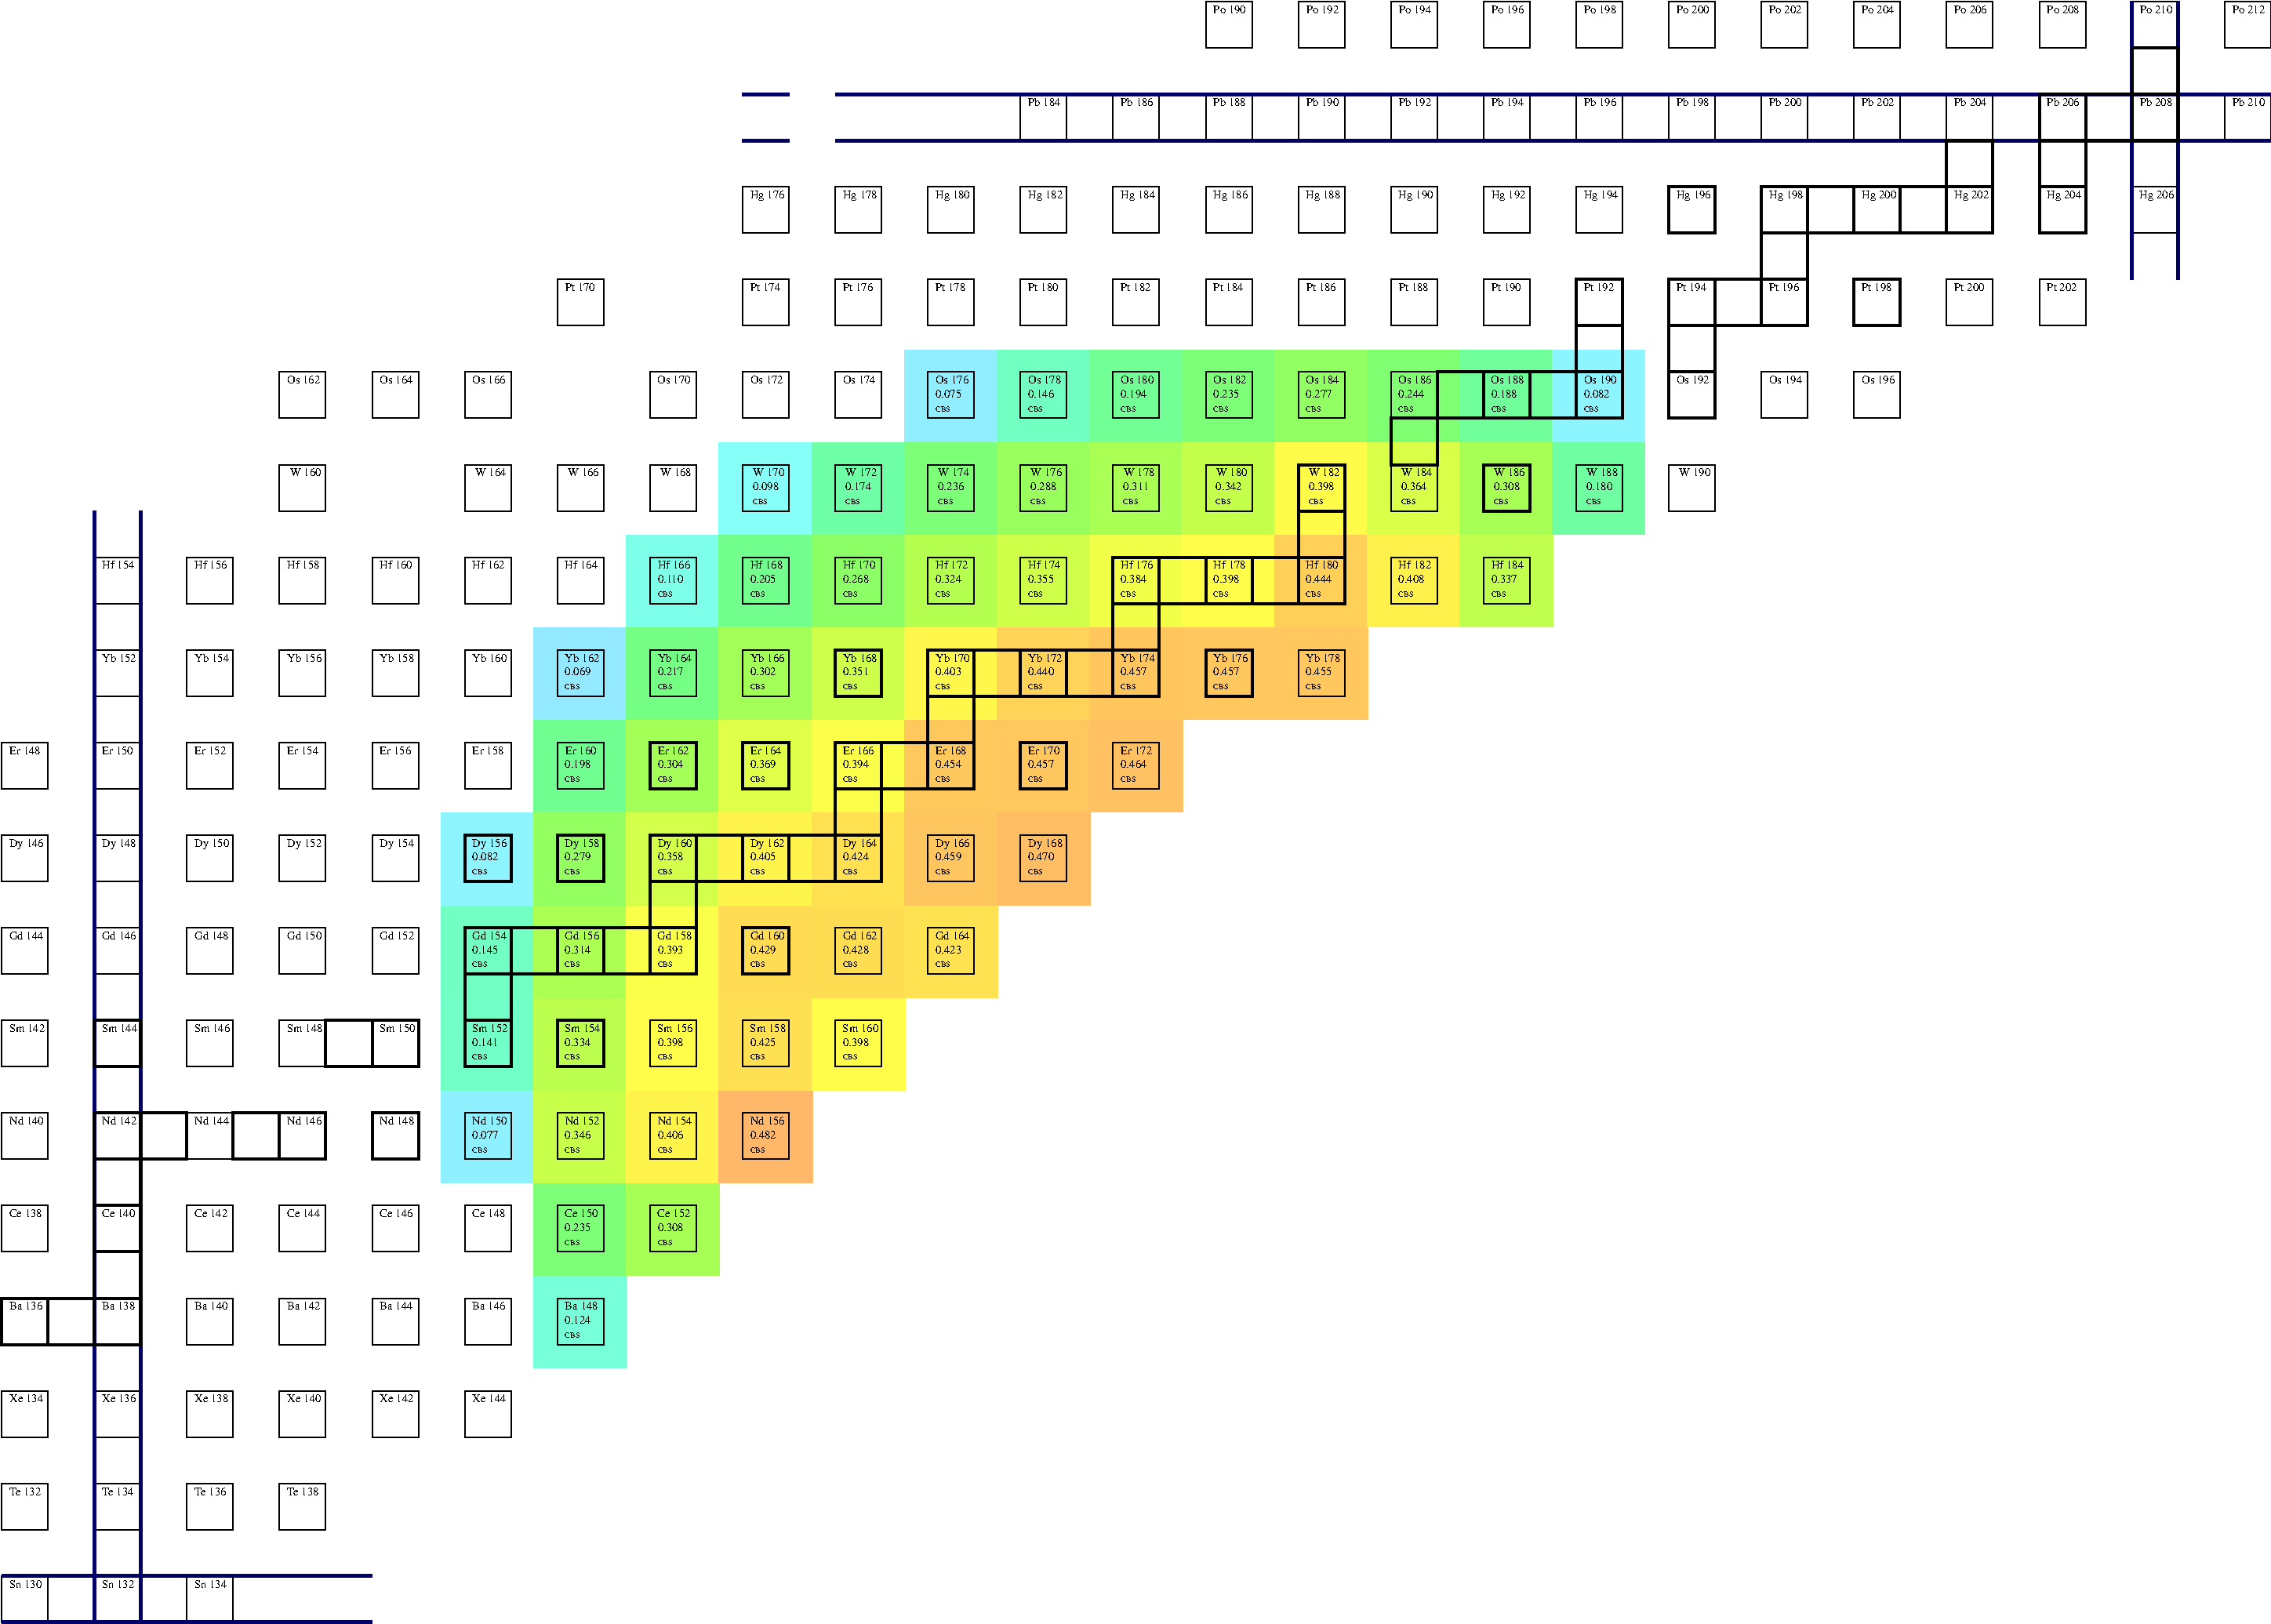
\includegraphics[width=\textwidth]{r_beta_chart.pdf} \label{CBSchart}
\caption{This is a part of the chart of nuclei. The colors correspond to the CBS structure parameter $r_{\beta}$. Each box is labeled with the values of $r_{\beta}$ and $B\cdot\beta_{\rm max}^2$.}
\end{figure}

\section{Installation}
Unpack the source tarball and enter the resulting directory by typing
\\~\\
\verb!tar -zxvf cbsmodel-1.0.tar.gz!
\verb!cd cbsmodel-1.0!
\\~\\
The Program makes use of the \textit{GNU scientific library} and the \textit{readline library}. If they are both properly installed on the system, you can compile the cbs source code by entering 
\\~\\
\verb!./configure! \\
\verb!make! \\
\verb!make install!  (as root)\\

\section{User Guide}
The program \textit{cbs} can be operated interactively, via command line arguments or with an input file.
\subsection{Interactive Mode}
To enter the interactive mode of \textit{cbs}, just type 

\verb!cbsmodel! \\
in the terminal. You should see a command prompt 

\verb!>>>! \\
and the program expects you to enter a command. If you want to describe a nucleus with nucleon number $A$ and proton number $Z$, you have to enter these two numbers. The current value of $A$ can be obtained by typing 

\verb!A! \\
(followed by carriage return). The program should answer with $168$ which is the initial value for $A$ as the program is started. You can modify this value (to $154$ for instance) by typing 

\verb!A 154! \\
(without \verb!=!). In the same way one can change every parameter of the program (see reference guide \ref{ReferenceGuide} for a list of all parameters). Let's go on by changing $Z$ to $62$ ($={\rm Sm}$). 

\verb!Z 62! \\
Now the program is set up to describe the nucleus $^{154}{\rm Sm}$. The example folder of the package contains a simple text file called \verb!154Sm.E! that contains a list of the experimentally measured ground state bands of $^{154}{\rm Sm}$. The content of the file is

\verbatiminput{../examples/154Sm.E} 
To reproduce the energy levels of a nucleus one wants to fit the two parameters $r_{\beta}$ and $B\cdot\beta_{\rm max}^2$ to the experimental data. This can be achieved by typing

\verb!fit 154Sm.E rb Bbm2! \\
Note that you must enter the correct path to the file \verb!154Sm.E! if it is not in the directory where you started the CBS program. The command should result in an output like this
\begin{verbatim}
0.1 0.01 (start)       
0.282357 0.0166837 (1) 
0.32491 0.0236887 (2)  
0.354007 0.0276625 (3) 
0.362122 0.0283363 (4) 
0.362537 0.028345 (5)  
0.36254 0.028345 (6)   
0.362539 0.028345 (7)  

Fit successful

rb    : 0.362539 +- 0.00320499
Bbm2  : 0.028345 +- 8.58551e-05
bmax  : 0.3 (fixed)
chi   : 0 (fixed)
E0    : 0 (fixed)
eps   : 0 (fixed)
bf    : 1 (fixed)
bs    : 0 (fixed)

reduced chisquare : 0.472668

                     CBS fit     data points       residues
--------------------------------------------------------------
  energy( 2 0 ) :    81.3513        82 +- 1      -0.648726
  energy( 4 0 ) :    266.246       267 +- 1      -0.754399
  energy( 6 0 ) :    544.376       544 +- 1       0.375804
  energy( 8 0 ) :     903.46       903 +- 1       0.459666
 energy( 10 0 ) :    1332.73      1333 +- 1      -0.274804
\end{verbatim}
After this, the parameters \verb!rb! ($=r_{\beta}$) and \verb!Bbm2! ($=B\cdot\beta_{\rm max}^2$) are updated as you can verify by typing 

\verb!rb! \\
or 

\verb!Bbm2! \\

To make some calculations, for instance the energy of the $12^{+}_1$ state, you can type

\verb!energy 12 0! \\
where the first number ($12$) is called $L$ and refers to the angular momentum of the state. The second number ($0$) is called $s$ and refers to the number of inner nodes of the $\beta$ part of the wave function. $s=0$ is the ground state band, $s=1$ is the $\beta$ band. Note that this is different from \cite{Pietralla} where $s=1$ is the ground state band, $s=2$ is the beta band and so on. You can display the $\beta$ part of the wave function by typing

\verb!wavedisp 12 0! \\
Note that this only works if you have \textit{Gnu plot} and \textit{Image Magic} installed on your system. Here you can see that the wave function indeed has no inner nodes. If you are more elaborate and want to calculate transition strengths, you also have to determine the parameter $\beta_{\rm max}$ (\verb!bmax! in the program). This you can do by fitting it to experimental data as given in the file \verb!154Sm.T! with the command

\verb!fit 154Sm.T bmax! \\
or you can fit all three parameters at the same time if you provide transition strengths and level energies together in one file ( as in 154Sm.ET ) with the command 

\verb!fit 154Sm.ET rb Bbm2 bmax! \\
All parameters given after the filename are fitted to the data. Fitable parameters are: \verb!rb Bbm2 bmax E0 eps bf bs!. You can not fit \verb!A! and \verb!Z!. Note that certain parameters are correlated to certain observables. Albeit possible, it doesn't make sense to fit these parameters if the corresponding data is missing in the data file.

Transition strength are usually given in units of ${\rm e}^2 {\rm b}^2$. If you want to switch to Weisskopf units, just type

\verb!Wu! \\
From now on, all transitions strength are given and read in W.U. Note that your data files for the fitting procedure now also have to provide numbers in W.U. for correct results. If you want back to ${\rm e}^2 {\rm b}^2$, type

\verb!noWu! \\
To calculate $B(E2)$ transition strengths from a state $L_1=6, s_1=1$ to another state $L_2=4, s_2=0$, type

\verb!BE2 6 1 4 0! \\
Sometimes one needs the $B(E2)$ transition matrix element. For the same transition this can be obtained by typing 

\verb!ME2 6 1 4 0! \\
To end the program you simply type 

\verb!exit! \\
To get an overview over all available commands type
\verb!help! \\

\subsection{Command Line Mode}
The exact same commands as in the interactive mode can be executed when they are passed as command line arguments. If you start the CBS program like this

\verb!cbsmodel A 154 Z 62! \\
You enter the interactive mode and the values for $A$ and $Z$ are already set up to work with $^{154}{\rm Sm}$. If you don't want to end up in the interactive mode you have to give \verb!exit! as the last of the command line arguments. For example just calculating the $2^{+}_1$ energy for the default parameters goes like this

\verb!cbsmodel energy 2 0 exit! \\
Fitting to experimental data, calculating a matrix element and exit goes like this

\verb!cbsmodel A 154 Z 62 fit 154Sm rb Bbm2 bmax ME 0 1 0 0 exit! \\
If you find the verbosity of the fitting annoying, you can spice the call with the \verb!simpleoutput! command

\verb!cbsmodel A 154 Z 62 simpleoutput fit 154Sm rb Bbm2 bmax ME 0 1 0 0 exit!

\subsection{Input File Mode}
Since \textit{cbs} reads its input from stdin, you can simply place all commands in one simple text file (each line contains one command) and start the program like this

\verb!cbsmodel < inputfile! \\
You can also combine command line usage with an input file.


\section{Reference Guide} \label{ReferenceGuide}
\subsection{Energy Levels}
The formula to calculate the energy CBS levels is
\begin{align}
E(L,s) = E_0 
     + \frac{z_{L,s}^2 - z_{L,s}^2}{2 \, B\cdot\beta_{\rm max}^2}
	 + \epsilon \cdot L\,(L+1)
	\quad \text{if $s\neq1$} \\
E'(L,s) = b_s \, (E(L,s)+b_s) \quad \text(else)
\end{align}
\subsection{Parameters}
the following parameters define the state of a \textit{cbs} session. The parameters listed first are the ``classical parameters'' that appear in \cite{Pietralla}. Default values (and units) at the start of the program are given in parentheses.
\begin{itemize}
\item \verb!A!: ($A$) number of nucleons ($168$)
\item \verb!Z!: ($Z$) number of protons ($70$)
\item \verb!rb!: ($r_{\beta}$) structure parameter $r_{\beta}$ ($0.1$)
\item \verb!Bbm2!: ($B\cdot\beta_{\rm max}^2$) energy scale parameter $B\cdot\beta_{\rm max}^2$ ($0.01 \hbar^2/{\rm keV}$)
\item \verb!bmax!: ($\beta_{\rm max}$) $B(E2)$ scale parameter $\beta_{\rm max}$ ($0.3$).
\end{itemize}
The following parameters are additional ones to extend the range of application of the model. One example for this is the description of super deformed bands with the CBS model. These Parameters are initially set to values that reproduce the behavior of the CBS model in \cite{Pietralla}.
\begin{itemize}
\item \verb!E0!: ($E_0$) energy of the ground state ($0.0 {\rm keV}$)
\item \verb!eps!: ($\epsilon$) fraction of rigid rotor admixture ($0.0$)
\item \verb!bf!: ($b_f$) energy factor for beta band ($1.0$)
\item \verb!bs!: ($b_s$) energy shift of the beta band ($0.0 {\rm keV}$)
\end{itemize}
\subsection{Commands}
A complete list of commands in the form 

\verb!commandname parametername<parrametertype> ...! \\
Parameters enclosed in brackets \verb![]! are optional. Parameters enclosed in curly braces \verb!{}! may occur once ore more often. The notation \verb!(A|B)! indicates that either \verb!A! or \verb!B! is needed.
\begin{itemize}
\item \verb!energy L<int> s<int>!: energy of level $(L,s)$
\item \verb!ME2 L1<int> s1<int> L2<int> s2<int>!: transition $E2$ matrix element from level $(L1,s1)$ to $(L2,s2)$
\item \verb!BE2 L1<int> s1<int> L2<int> s2<int>!: $B(E2)$ transition strength from level $(L1,s1)$ to $(L2,s2)$
\item \verb!rho2E0 L1<int> s1<int> L2<int> s2<int>!: $\rho(E0)$ transition strength from level $(L1,s1)$ to $(L2,s2)$
\item \verb!fit ( filename<string> | begindata DATA enddata ) { parameter<param> }!
\item \verb!store filename<string>!
\item \verb!load filename<string>!
\item \verb!Wu!
\item \verb!noWu!
\item \verb!simpleoutput!
\item \verb!fulloutput!
\item \verb!wavedat!
\item \verb!waveeps L<int> s<int> filename!
\item \verb!wavedisp L<int> s<int>!
\item \verb!help!
\item \verb!license!
\item \verb!exit!
\end{itemize}



\begin{thebibliography}{99}
\bibitem{Pietralla} 
N. Pietralla and O. M. Gorbachenko, Phys. Rev. C {\bf 70}, 011304(R) (2005).
\bibitem{Iachello} 
F. Iachello, Phys. Rev. Lett. {\bf 87}, 052502 (2001).
\end{thebibliography}

\end{document}
